\section{Q5Cost library}

In the deployment of a common suite of codes, a standard file format is
necessary.  A first attempt in file standardization has been made in
Toulouse with the COST format. This format has been also implemented in most
of the Ferrara suite.

The format is made of four files, each one with a different extension:
\begin{itemize}
\item \texttt{.Mono}, a binary file containing the atomic basis set overlap and the one-electron
integrals on the molecular orbital basis set
\item \texttt{.ijcl}, a binary file containing the two-electron integrals
on the molecular orbital basis set
\item \texttt{.Info}, a cleartext file containing namelists describing various
metainformation, like the number of active orbitals, the nuclear
repulsion energy, the geometry and so on
\item a file called \texttt{INPORB}, containing the molecular orbitals. The format is
the same provided by the \molcas program, enriched with additional
information needed by the Toulouse suite of programs.
\end{itemize}

The COST files are written using the standard sequential access provided by
\texttt{READ} and \texttt{WRITE} statements in Fortran. No
{intention-revealing} interfaces are provided for accessing the data. This
implementation, although simple to manage, is limited in a lot of points:

\begin{itemize}
\item the standard sequential access provided by Fortran imposes to agree
on data size, data ordering, and chunking. It does not allow random access,
making difficult to update already written information, or to posticipate
the writing operation of some entity. It complicates reorganization
or expansion of the stored information set
\item files are not platform independent. A file written on an Intel
x86 machine is unreadable by an IBM SP4 supercomputer, and viceversa. This
limits the output sharing
\item it is difficult to access the stored information in a clear
representation. This is a major issue when debugging computational chemistry
codes. At the moment the access is through ad-hoc visualizers or hexadecimal
editors
\item the file is difficult to split, merge, compare, or describe with
metainformation
\item the API for accessing the file format is limited in features,
allowing no basic consistency checks or a clean interface. Documentation 
is written as code comments. This makes difficult to direcly access the
information.
\end{itemize}

Q5Cost is a library devoted to solve these problems. Based on the
{platform-independent} file format HDF5, Q5Cost allows the user to produce binary
files through a well documented interface. The library also takes care of
providing useful information during debug, explicitly stating inconsistent
data or wrong usage of the routines.

\subsection*{HDF5 file format}

As defined on the website\cite{hdf5-site}, ``HDF5 is a general purpose library and file
format for storing scientific data''. HDF5 targets the data management needs
of scientists and engineers working in high performance, data intensive
computing environments. This is achieved by providing an efficient library and
file format, specifically tuned to read and write binary data efficiently.

A HDF5 file appears to the user as a single file containing a structured
graph of entities. This structure is conceptually very similar to a UNIX
filesystem, and is defined by means of three entities: \textit{Groups},
similar to directories, \textit{Datasets}, similar to files
and \textit{Attributes}, similar to metainformation such as permissions and
owner.  Data are stored into Datasets and Attributes, and can be organized
with Groups. The HDF5 library provides an interface to handle these
entities.

The most striking feature of HDF5 is the platform independence of the files.
A file written on a 32 bit Little Endian architecture (like, for example, an
Intel x86 machine) can be transferred and read transparently on a 64 bit Big
Endian machine (like, for example, the IBM SP4) or a 64 bit Little Endian
machine (like an IA64 machine). This is of critical importance
in grid environments, where heterogeneity is the rule, rather than the
exception.

Another important feature of HDF5 is the suite of utilities, which allows the
user to find differences between two HDF5 files, obtain a textual dump of
Groups, Datasets and Attributes layout (resembling the ``ls'' program in
UNIX environment) or a more detailed view presenting also the numerical
data.  This simplifies the access to this information, which is critical
in the debug phase.

The HDF5 library is made of a directly accessible C layer. Alternative APIs
are available for C++, Fortran 90, and Java. The library is actively
developed, is free and released as open source software.

\subsection*{Q5Cost file format and library} 

The Q5Cost library is implemented on top of the HDF5 library.  It provides
read and write access to HDF5 files with a specifically designed high-level
interface for quantum chemistry developers. 

The rationale is to provide a Fortran interface based on well known chemical
entities, rather
than groups or datasets like in the HDF5 interface. HDF5 takes care of
low-level management of the file, and Q5Cost provides the high-level
API to store and retrieve chemical entities.

An extensible data model has been rationalized thanks to the knowledge
obtained by the involved researchers. Some firm points have been
discovered.

The first point is that many different types of simple and small data
must be handled. Some examples are nuclear energy, molecular orbital labels,
molecular symmetry and so on. We will refer to these data as
\textit{metadata}, in order to distinguish them from the real large
information on the chemical system, the integral values.

Metadata represents well-known chemical entities and belong to three
generic data classes: \textit{Scalars}, \textit{Vectors} and
\textit{Matrixes}. For example, the nuclear repulsion energy is a floating
point scalar, molecular orbitals can be represented as a (N,M) floating point matrix, the
associated orbital energies is a floating point vector, the molecular
orbital labels is a vector of strings and so on. The library should provide
an interface for accessing these data, both as generic or specialized
entities.

A second point is the fact that in quantum chemistry large sparse
matrixes with an arbitrary number of indexes (rank-$n$ arrays) are very
common data structures. These data usually scale aggressively with the
system size, and they are normally accessed with a chunked sequential approach.
This is the case of entities like two-electron integrals, or atomic
orbitals overlap, but also much other more application-specific
information, like the four-particles density matrix.

The sparse nature of these matrixes encourages to store only non-zero
elements, each one associated to $n$ indexes in the case of a rank-$n$
array. This representation of the data, although not always efficient in
term of space occupation, is well known by the interested parties, easy to
debug and already integrated in the current codebase both for memory
representation and file storage. The library structure allows 
future expansions of the low-level storage format, in order to reduce the
storage needs, but in the first development phase this issue has not
been investigated, and the current format is useful for the direct debug of
the file.

These large data arrays share common features:
\begin{itemize}
\item they usually are integrals, whose evaluation involves one
operator and a given number of functions. These functions are
referred by the indexes of the matrix. For example, two-electron integrals
on the molecular orbital basis are stored as a rank-4 array with indexes
referring to the molecular orbitals. In the case of atomic basis set overlap
integrals, the indexes refer to the atomic basis set
\item the rank of the array depends on the physical meaning of the
integrals. Atomic basis set overlap is described by two indexes, and can be
stored as a rank-2 array. Two-electron integrals have four indexes imposing a
rank-4 array and the four-particles density matrix has eight indexes,
requiring a rank-8 array
\item additional information is needed to describe the involved operator
(for example its symmetry) and the entities the indexes refer to.
\end{itemize}

All this information can be classified under a generalized \textit{Property}
concept, which is described by the matrix rank and the definition of the
involved operator and functions. Integrals are stored by means of a
dedicated abstraction, named \textit{CompactMatrix}, enriched with
metadata to define the Property, like its name, rank, symmetry and
real/complex nature.

Some properties are well-known chemical entities, and chemists are
used to refer to them by name. A specific library access has been provided
to handle these entities, easing the need to specify well-known information
about them.

A further step is to recognize containment relationships and simple
consistency patterns between the involved entities. A graphical
representation can be seen in Fig. \ref{fig:q5cost-schema}.

\begin{center}
\begin{figure}[ht]
\begin{center}
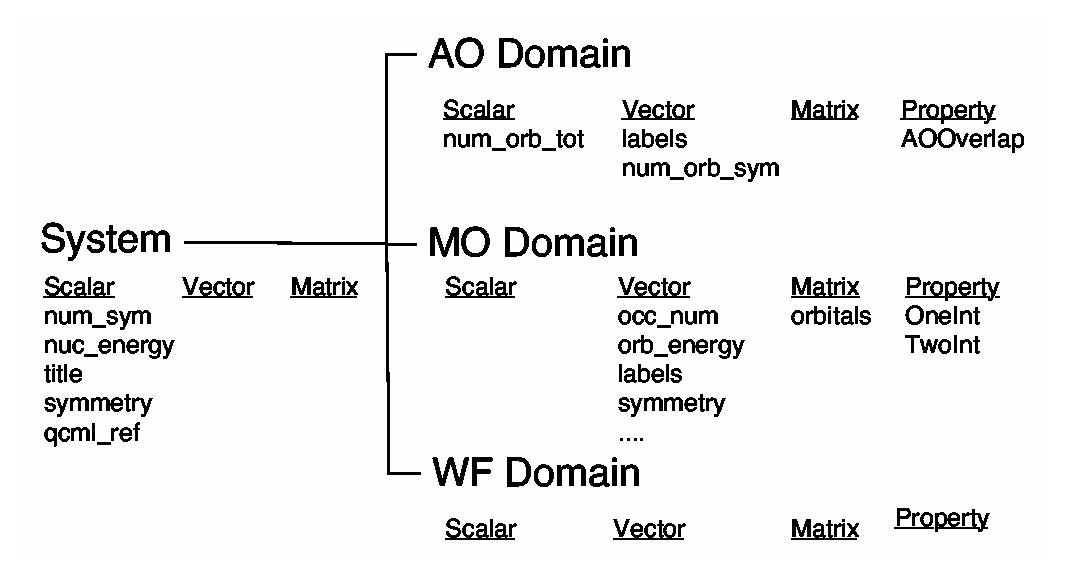
\includegraphics[width=10cm,keepaspectratio]{04_grid/images/q5cost-schema-gimped.eps}
\end{center}
\caption{\footnotesize A graphical representation of the containment
relationship between the System and the Domains. Specific metainformation is also
presented, classified under the appropriate environment.
}
\label{fig:q5cost-schema}
\end{figure}
\end{center}


The first high-level logical container is the \textit{System} object. This
object represent a molecular system as described by its structural
informations, such as symmetry and atomic coordinates, and also contains all
the metadata that are invariant at this level, like for example nuclear
repulsion energy, or a title. Multiple Systems make possible to handle
different molecular geometries.

A System can contain several \textit{Domains}. The role of a Domain is to
group together Properties whose indexes conceptually refer to the
same entity. Three Domains have been recognized as fundamental: \textit{AO}
for Atomic Orbital, \textit{MO} for Molecular Orbitals and \textit{WF} for
Wavefunction.  Each Domain can contain an arbitrary number of Properties, and
additional metadata represented as specialization of Scalar, Vector and Matrix
entities.

The AO Domain holds Properties whose indexes refer to the atomic basis set
funtions: overlap, one-electron and two-electron integrals on the atomic
basis set are some examples, in addition to the generic Property. The
associated metadata hold information about the atomic orbitals, like their
number, labels and symmetry.

The MO Domain holds Properties referring to molecular orbitals:
one-electron and two-electron integrals on the MO basis set are examples, in
addition to the generic Property. The descriptive metadata refer to the
molecular orbitals, their number, labels and symmetry, the AO
basis they were derived from, orbital energies, classification and
occupation numbers.

The WF Domain holds Properties referring to the electronic states. At the
moment a complete definition of this Domain is not available and not
subjected to major research and development, given its non-critical nature
for the first deployment of the library.

Each Domain can be defined under different occurrences, by means of a textual
identifier (\textit{tag}) chosen by the user, with a default value if no tag is
provided. The aim is to provide storage of multiple entries for each Domain,
like in case of multiple molecular orbitals in the MO Domain, or multiple
basis sets in the AO Domain.

\subsection*{Library structure}

The library is written in Fortran 95 and is made of different modules, each
one providing different facilities. The most important modules are

\begin{itemize}
\item \textit{Q5Cost}: defines the high-level API, providing
subroutines designed to be accessible from the final programmers of the
laboratories involved in the project
\item \textit{Q5Core}: provides a wrapping facility for HDF5 routines, in order to
perform additional useful services like reference counting and debugging.
Also provides simplified routines to perform frequently used low-level
tasks
\item \textit{Q5Error}: provides facilities for high-level debugging of the
library and client codes. This module implements a ring buffer for error
messages, different logging levels, generic reference counting for catching
leaks of HDF5 references, and a subroutine call stack trace.
\end{itemize}

Subroutines for each module have been namespaced with an appropriate prefix,
and names have been chosen to provide an explicit and {intention-revealing}
interface to the entities described in the previous section.  

Although Fortran 95 does not allow object oriented (OO) programming, some OO
concepts have been used in the development of the library, keeping into
account the procedural programming background of the final developers. The
state is preserved into the HDF5 file, and subroutines refer to the file
directly through the HDF5 identifier, a more easy concept for Fortran
programmers used to unit descriptors.

\subsubsection*{The Q5Cost module}

This module is the main reference for the final users. It provides
subroutines to read and write HDF5 files in the Q5Cost format with a high-level
abstraction. The users can deal with high-level concepts without worrying
about low-level implementation details. If a finer access is needed to the
underlying HDF5 file, the Q5Core module provides this access in a simpler
way with respect to raw HDF5 routines.

The Q5Cost module is made up of routines belonging to the following
classes:
\begin{itemize}
\item \textit{File}: create, open, close the file and write/read root
metainformation, like creation time, access time and file version
\item \textit{System}: create or check the existence of the System and set/get
its metainformation
\item \textit{AO}: create or check the existence of the AO Domain and set/get its
metainformation
\item \textit{AOOverlap}: create, read and write data for the atomic basis set
overlap Property
\item \textit{MO}: create or check the existence of the MO Domain and set/get its
metainformation
\item \textit{MOOneInt}: create, read and write data for the one-electron
integrals in molecular orbitals basis
\item \textit{MOTwoInt}: create, read and write data for the two-electron
integrals in molecular orbitals basis
\item \textit{WF}: create or check the existence of the WF Domain and set/get its
metainformation. Still experimental and mostly unimplemented.
\end{itemize}

Additional routines are provided for generic access to the Property
class, allowing to manage generic property data. Subroutines for
AOOverlap, MOOneInt and MOTwoInt delegate calls to these Property routines,
automatically passing well-known parameters about the involved property.

Q5Cost module routines provide a context-based access to chemical
entities. This access is transformed into a path-based access, creating
an appropriate layout for HDF5 groups, datasets and attributes, and
writing the user-provided data on the file. Some data are automatically
written by the library, like the creation or access time and the
Q5Cost library version. 

One important aspect of this format is that the user is not forced to
produce information for all quantities. The user can store only those
quantities that are actually available.  Constraint checks are however
mandatory in order to assure basic file consistency. For example, no MO
Domain can be created if a System and an AO Domain have not been provided,
in order to guarantee the presence of fundamental data, like the number of
symmetry species and the number of basis functions for each symmetry
species.

\subsubsection*{The Q5Core module}

The Q5Core module is a low-level module designed to provide wrapping
facilities between the Q5Cost library and the HDF5 library. At the moment it
is focused at providing additional debug information, reference counting
for HDF5 objects, additional low-level API to simplify common tasks.

This module also provides path-based creation of Scalar, Vector and
Matrix entities (in contrast with the context-based approach of the Q5Cost
module, which focuses on chemical concepts rather than HDF5 paths) and also
routines to ease handling of the Property index/value data, relative to the
CompactMatrix class. Most of the Property routines accessing index/value
data delegate to CompactMatrix subroutines. 

Q5Core module could also be useful to guarantee transparency toward a
low-level format migration from HDF5 to other storage formats. This could
allow the Q5Cost module to remain unchanged and unaware of the final
low-level format, but in the current deployment this was not a priority.
Final users are not expected to access Q5Core module routines, except for
highly experimental tasks.

\subsubsection*{The Q5Error module}

The Q5Error module provides subroutines to monitor the behavior of the
library and the client code. A ring buffer is provided to keep track of
error messages generated by the library. A verbosity level can be set from
totally silent to highly verbose, where each subroutine call and return are
reported into the buffer. Also, a stack for backtracing has been implemented
to keep track of the call tree. The tree is printed out when an error occurs
and error reporting is requested. 

Different specific error codes have been devised to report anomalous
behavior to the client code or to the library itself. Error codes are
defined as numeric parameters and report situations ranging from invalid
parameters to non-existence of some information into the file. The presence
of an error condition is reported to the client code through the last
parameter of each subroutine.

\subsubsection*{Additional details: testsuite and documentation}

A dedicated module for testsuite deployment and a set of tests have been
implemented to stress the library through a high number of well-known
critical situations, evaluating the correctness of the response. At the
moment, more than 300 tests are implemented, covering the most common usage
patterns. Reference counting is checked to prevent leaks of HDF5
references. The testsuite provides an effective watchdog for debugging,
refactoring, and bugfixing.

Library documentation is embedded into the Fortran code as comments,
using a custom markup system.  A simple parser, written in the
Python\cite{python-site} programming language, extracts the documentation
producing HTML files.
